% Paper template for TAR 2021
% (C) 2014 Jan Šnajder, Goran Glavaš, Domagoj Alagić, Mladen Karan
% TakeLab, FER

\documentclass[10pt, a4paper]{article}

\usepackage{tar2021}

\usepackage[utf8]{inputenc}
\usepackage[pdftex]{graphicx}
\usepackage{booktabs}
\usepackage{amsmath}
\usepackage{amssymb}
\usepackage{hyperref}

\title{Can text augmentation augment commonsense knowledge?}

\name{Marko Čuljak, Darijo Brčina, Vedran Kolka}

\address{
University of Zagreb, Faculty of Electrical Engineering and Computing\\
Unska 3, 10000 Zagreb, Croatia\\ 
\texttt{\{marko.culjak,darijo.brcina,vedran.kolka\}@fer.hr}\\
}

\abstract{
Learning commonsense knowledge is a difficult task for machines. However, with the recent advent of transformer models, the ability of NLP systems to learn commonsense knowledge has significantly improved. Motivated by the lack of attention to text augmentation approaches in tackling this challenge, in our research, we experiment with several text augmentation techniques, including a task-specific GPT-2-based technique. We train multiple models in order to explore the effect of text augmentation on the performance of commonsense knowledge validation systems. Our best model yields results comparable to state-of-the-art, with an accuracy of 95.6\% on the SemEval-2020 Task 4, Commonsense Validation, subtask A test set.
}

\begin{document}

\maketitleabstract

\section{Introduction}

Most adult humans are equipped with common sense i.e., according to Cambridge Dictionary, the ability to use good judgment in making decisions and to live in a reasonable and safe way. Even though commonsense knowledge is mostly basic, it is not a fundamental principle of the Universe but rather a collection of knowledge built by generations of humans through observations of phenomena in their surroundings. Since humans are not born with common sense, they start learning it from the earliest stages of their life, either explicitly or implicitly.

On the other hand, teaching computers commonsense knowledge is a difficult task. This is primarily due to two reasons: (1) unlike humans, machines are unable to learn implicitly or passively and (2) commonsense knowledge is broad and constantly evolving. Yet, recently, with the advent of transformer models \citep{transformers}, the ability of NLP systems to learn commonsense knowledge has improved significantly. The approaches based on fine-tuning transformer models previously pre-trained on large text corpora continuously achieve state-of-the-art results on natural language understanding (NLU) tasks. However, not much attention has been paid to text augmentation, especially in NLU tasks.

In this paper, we tackle the first subtask from SemEval-2020 Task 4, Commonsense Validation and Explanation (ComVE) \citep{wang-etal-2020-semeval} by employing several text augmentation techniques. We explore the effect of these techniques on the performance of common sense validation systems. We experiment with back translation and contextual embeddings-based data augmentation techniques. Furthermore, we propose a text augmentation technique that leverages a GPT-2 model \citep{radford2019language} to generate artificial data. The subtask on which we evaluate the models' performance requires them to identify which of the given two sentences does not make sense. For example, for the following two sentences:\\
$s_0:$ \textit{He poured milk on his cereal}.\\
$s_1:$ \textit{He poured orange juice on his cereal}.\\
the desired output of the model is $1$ because the sentence $s1$ is against common sense. The data provided as a part of the task is described in Section \ref{data} The systems, along with text augmentation techniques we experimented with are described in detail in Section \ref{model} and Section \ref{aug}, respectively. Finally, in Section \ref{results}, we present the results of the experiments.


\section{Related work}
\label{sec:rw}

In recent years, many approaches tackle common sense-making and reasoning leveraging transfer learning and transformer models. \citet{wang-etal-2019-make} present promising results on common sense-making and not as promising results on common sense reasoning. The authors state that the results show that sense-making remains a technical challenge for such models, whereas inference is a key factor that is missing. Nevertheless, the results are meaningful because they show that artificial intelligence systems are still far from human-like performance in common sense reasoning.

The most successful approaches to the Validation subtask \citep{zhang-etal-2020-cn,zhao-etal-2020-ecnu} leverage pre-trained transformer-based models and external commonsense knowledge stored in the ConceptNet \cite{conceptnet}. However, as stated by \citet{wang-etal-2020-semeval}, the success of the ConcepNet-based systems may be attributed to the data leakage which may have occurred because ConceptNet was used as an inspiration for ComVE data generation along with transformer-based models. Rather than leveraging the existing knowledge bases, we attempt to generate additional knowledge artificially by employing text augmentation techniques.

Two approaches at ComVE employed back translation to enhance their common sense validation model performance \citep{liu-etal-2020-lmve,jon-etal-2020-fit}. Although they reported an improvement over their baselines, they do not back their results with statistical significance testing. As for GPT-2 artificial data generation, our approach is inspired by \citet{kumar-etal-2020-data}.


\section{Dataset}
\label{data}
ComVE subtask A dataset includes 10000 sentence pairs in the training set, 997 samples in the validation set, and 1000 samples in the test set. The distribution of labels is balanced. The average word count of sensical and nonsensical sentences in the training, validation, and test set is given in Table \ref{lengths}.
\begin{table}[]
    \caption{The average word counts of sensical and non sensical sentences.}

    \begin{center}
    \begin{tabular}{cccc}
        \toprule
        & Training & Validation & Test\\
        \midrule
        Sensical & 7.67 & 7.12 & 7.25\\
        Nonsensical & 7.69 & 7.16 & 7.36 \\
        \bottomrule
    \end{tabular}
    
    \end{center}

    \label{lengths}
\end{table}

\section{Common sense validation model} 
\label{model}
Our system consists of a pre-trained transformer model as a sentence encoder which is followed by a dropout layer, a linear layer, and a softmax layer. The linear layer is used to map the sentence encoder's output to a single score value. The softmax layer is used as a score comparator. The architecture of the proposed system is visualized in Figure \ref{fig:model}.

As encoders we used the following transformer models: DistilBERT$_{\text{BASE}}$ and DistilRoBERTa$_{\text{BASE}}$ \citep{distil-bert}, ALBERT$_{\text{BASE}}$ \citep{albert}, ELECTRA$_{\text{SMALL}}$ and ELECTRA$_{\text{BASE}}$ \citep{electra}. Due to resource limitations we optimize the hyperparameters only on the model based on ELECTRA$_{\text{SMALL}}$ and reuse the obtained hyperparameters on other transformer-based models. For the same reason we do not consider the largest versions of the aforementioned transformers. Aside from transformers we also experimented with a Bidirectional LSTM (BiLSTM) \citep{schuster1997bilstm} as the encoder.

\subsection{Implementation details}

The transformer models were downloaded through HuggingFace transformers \citep{wolf-etal-2020-transformers} module. Fine-tuning of our model was done using Pytorch Lightining\footnote{\href{https://github.com/PyTorchLightning/pytorch-lightning}{https://github.com/PyTorchLightning/pytorch-lightning}} framework in Google Colab\footnote{\href{https://colab.research.google.com/}{https://colab.research.google.com/}} environment.

We trained our models using the AdamW optimizer. After a grid search hyperparameter optimization with respect to the provided validation corpus, we concluded the optimal parameters for the AdamW optimizer are 4e-5 for the learning rate, and 1e-2 for the weight decay. We used a linear scheduler with warm-up for adjusting the learning rate during training and we set the number of warm-up steps to correspond to one epoch. Following the same hyperparameter optimization procedure, we concluded that the optimal batch size is 32. As for the dropout layer, we set drop probability for systems trained solely on original data and data augmented by employing back translation and contextual embeddings to 0.1, while for systems that leverage data generated by GPT-2 we set the drop probability to 0.8. We trained our models through 8 epochs, saving the best model with respect to validation loss.

Since the BiLSTM-based model performed poorly on the validation set, we were unable to find hyperparameter values that stand out. We settle for an architecture with 2 BiLSTM layers, a hidden size of 300, a learning rate of 5e-4, and weight decay of 1e-2. As for word representations, we use 300-dimensional GloVe embeddings \citep{pennington2014glove}.


\begin{figure} 
    \centering
    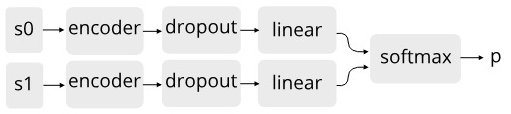
\includegraphics[width=8.5cm]{images/model14.jpg}
    \caption{The system architecture used in all experiments. The \textit{encoder} is either a transformer or a BiLSTM and \textit{p} denotes the predicted probability that $s0$ is against common sense given $s0$ and $s1$ as inputs.}
    \label{fig:model}
\end{figure}

\section{Text augmentation}
\label{aug}
Classic text augmentation techniques are based on deletion, addition, and replacement of certain words as well as changing the word order. Such techniques are not useful for NLU tasks because they may render sensical sentences nonsensical and vice versa. For example, if we change the word order in a sentence \textit{A man eats a cake.} we may end up with a sentence \textit{A cake eats a man.}, which is obviously against common sense. On the contrary, techniques based on alternating single letters in a text are also not particularly useful for NLU tasks since they do not modify the text in a manner significant enough to create new knowledge, although they may contribute to the robustness of a system to spelling errors, which is not essential for such tasks.

However, techniques such as back translation (BT) and replacement of certain words based on contextualized word embeddings (CWE) do not affect the sense of the sentences in a strong manner and may be able to generate additional knowledge, which is why we find them worth exploring. Aside from only modifying the provided data, we attempt to generate artificial sentence pairs by leveraging a GPT-2 model fine-tuned on the provided training data.

We used NLPAug\footnote{\href{https://github.com/makcedward/nlpaug}{https://github.com/makcedward/nlpaug}} library to perform back translation and CWE-based text augmentation and HuggingFace transformers to obtain the GPT-2 model. After obtaining the artificially generated datasets, we concatenated them to the original corpus, removing the duplicated pairs.


\subsection{Back translation}
The back translation text augmentation technique leverages two machine translation models: (1) a model that translates text written in language $A$ to language $B$ and (2) a model that translates the obtained text back from language $B$ to language $A$. The main motivation for back translation is the fact that texts may have multiple valid translations. In this work, we choose German as a language $B$.

\subsection{Contexutalized word embeddings}
\label{cwe}
CWE text augmentation leverages contextualized word embeddings to find a replacement of a word based on its surroundings. The hyperparameters of CWE text augmentation are thoroughly described in NLPAug's documentation\footnote{\href{https://nlpaug.readthedocs.io/en/latest/augmenter/\\word/context\_word\_embs.html}{https://nlpaug.readthedocs.io/en/latest/augmenter/word/\\context\_word\_embs.html}}. In this work we use BERT$_{\text{BASE}}$ for computing the CWE. We modified only one word in each sentence in a pair and set \texttt{top\_k} to 30 and \texttt{temperature} to 0.2. The \texttt{top\_k} and \texttt{temperature} parameters are selected by performing a grid search and manually evaluating the quality of 20 generated sentences.

\subsection{GPT-2}
Our approach in leveraging GPT-2 for text augmentation can be broken down into four phases: (1) fine-tuning, (2) generation\footnote{The code for fine-tuning and generation phases is the adaptation of \href{https://github.com/prakhar21/TextAugmentation-GPT2}{https://github.com/prakhar21/TextAugmentation-GPT2}. Due to resource limitations we were unable to perform hyperparameter optimization for fine-tuning so we used the hyperparameters proposed by the author.}, (3) preprocessing, and (4) selection.

\textbf{Fine-tuning.} Firstly, we fine-tune the GPT-2$_\text{MEDIUM}$ model on the corpus of concatenated sentence pairs obtained from the ComVE training dataset. Each text in the corpus begins with an "S:" string to denote the start of a text, followed by a sensical sentence, "/" token, a nonsensical sentence, and the "\textless$\vert$ endoftext $\vert$\textgreater" token. We fine-tune the model for 3 epochs, with a learning rate of 2e-5 scheduled by the cosine scheduler with warm-up with 300 warm-up steps, and with the batch size of 32.

\begin{table}[t]
    \caption{Accuracies(\%) of GPT-2$_\text{LARGE}$ with harmonic mean (HM), arithmetic mean (AM), geometric mean (GM), product (Prod) aggregation methods on the validation set. The best two results are in bold.}
    \begin{center}
        

    \begin{tabular}{cccc}
    \toprule
         HM & AM & GM & Prod\\
         \midrule
           65.0 & 66.4 & \textbf{74.9} & \textbf{78.8}\\
          \bottomrule
    \end{tabular}

    \label{tab:LM}

    \end{center}
\end{table}

\textbf{Generation.} In the generation phase we use the fine-tuned model to generate three times as many sentence pairs as the size of the training dataset (30k sentence pairs). For text generation, we use nucleus sampling \citep{nucleus}. This sampling technique randomly selects the next token from the smallest pool of tokens whose cumulative probability exceeds \texttt{p}, a hyperparameter which we set to 0.9. To avoid selecting words with extremely low probabilities for the sensical sentence we initially limit the pool size to at most 50 words. After the "/" token is generated we increase the pool size to 100 in order to increase the variability of possible tokens for the nonsensical sentence. The mentioned hyperparameters were selected based on the quality of generated sentences, similarly to the procedure mentioned in Section \ref{cwe}

\textbf{Preprocessing.} The preprocessing phase can be further broken down into 4 steps: (1) elimination of texts that do not match the structure of a valid sentence pair, (2) removing the texts which consist of the same sentences, (3) removing the pairs which are already a part of the ComVE training dataset, and (4) extracting the sentence pairs from the texts. In the first preprocessing step we remove all the texts that contain three or more sentences, texts that contain sentences with characters other than numbers, letters, and punctuation, or with two or fewer tokens. To tokenize the sentence and obtain the number of tokens we use GPT-2$_\text{LARGE}$ tokenizer.

\textbf{Selection.} To perform selection of the generated pairs we leverage GPT-2$_\text{LARGE}$ model. However, in this phase, we use it without fine-tuning. Firstly, we use lm-scorer\footnote{\href{https://github.com/simonepri/lm-scorer}{https://github.com/simonepri/lm-scorer}} to assign scores to all generated sentences. The sentence score is calculated by aggregating token probabilities computed by GPT-2$_\text{LARGE}$. We consider four aggregation methods: arithmetic mean, geometric mean, product, and harmonic mean. In further research we use only the geometric mean and product, producing two datasets which we denote by GPT-2-G, and GPT-2-P, respectively. The aggregation methods are selected based on the performance of the method on the validation set. To calculate the performance of aggregation methods we firstly calculate the sentence scores using GPT-2$_\text{LARGE}$ that employs a certain method. We then assign the labels to match the index of a sentence with a lower score. To measure the performance we use the accuracy score. Comparison of the performances is shown in Table \ref{tab:LM}. The product scoring achieved the best accuracy. This may be attributed to the fact that nonsensical sentences are slightly longer in all the datasets, as shown in Table \ref{lengths}. Since the token probabilities are in the interval $[0, 1]$, their product decreases with respect to sentence length. Therefore, sentences with fewer tokens are scored higher than longer sentences. On the contrary, other methods calculate some form of mean values, which leads to equal treatment of the sentences, regardless of their length.

\begin{table}[t]
    \caption{Word count means of the first 5k artificially generated sentences in GPT-2-G and GPT-2-P datasets. The average sentence lengths for the GPT-2-G are similar to those of the original training set.}
    \begin{center}
    \begin{tabular}{ccc}
        \toprule
        & GPT-2-P & GPT-2-G \\
        \midrule
      Sensical & 4.79 &  8.34 \\
      Nonsensical & 5.00 & 7.82 \\
      \bottomrule
    \end{tabular}
    \end{center}
    \label{tab:gptlen}
\end{table}


\begin{table*}[ht]
      \caption{The accuracies (\%) of models based on different encoders trained on the original dataset and the datasets generated by employing different text augmentation techniques. The amount of training examples in each dataset is shown in the brackets. \#$\theta$ denotes the number of parameters of each encoder. In the "Ensemble" column we report the results of the voting ensemble of models in the corresponding row. The best results in each row are in bold.}
    \begin{center}
        
    \begin{tabular}{cccccccc}
        \toprule
         Model & \#$\theta$ & Original (10k) & GPT-2-P (15k) & GPT-2-G (15k) & BT (18k) & CWE (20k) & Ensemble \\
        \midrule
        BiLSTM & 3.6M & 61.2 & 63.4 & 62.5 & 62.9 & 61.4 & \textbf{64.6}\\
        ALBERT & 11M & 82.8 & 81.7 & 80.6 & 82.4 & 82.3 & \textbf{83.8} \\
        DistilBERT & 110M & 84.8 & 86.1 & 85.7 & 84.0 & 85.3 & \textbf{86.4} \\
        DistilRoBERTa & 82M & 85.7 & 85.2 & 85.9 & 85.6 & 86.2 & \textbf{87.0}\\
        ELECTRA$_\text{SMALL}$ & 13M & 89.0 & 89.6 & 89.4 & 89.1 & 89.0 & \textbf{90.1} \\
        ELECTRA$_\text{BASE}$ & 110M & 95.0 & 93.7 & 94.6 & 94.7 & 94.6 & \textbf{95.6} \\
        \bottomrule
    \end{tabular}
  \end{center}
    \label{table:results}
\end{table*}



Finally, we select 10k sentence pairs ranked by the highest difference between the scores assigned to a sensical and a nonsensical sentence. However, we evaluate only the models trained on top 5k artificially generated pairs concatenated to the original data since they achieve the best results on the validation set in comparison to using the top 2.5k or 10k artificially generated pairs. After the selection is performed, we randomly shuffle the sentences in each pair and assign the labels accordingly. 

Mean word counts in each of the datasets are shown in Table \ref{tab:gptlen}. As expected, due to the nature of the aggregation methods, GPT-2-P contains shorter sentences on average in comparison to GPT-2-G. Figure \ref{fig:cum} shows the trends in mean word count in sentence pairs with respect to the number of selected sentences.

\begin{figure}
    \centering
    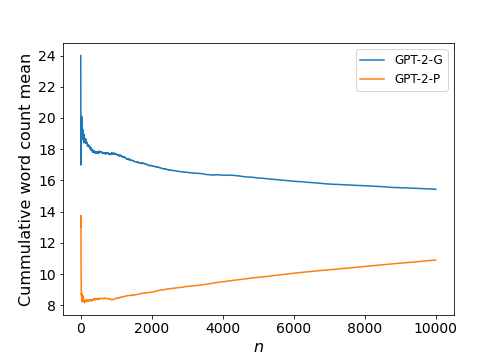
\includegraphics[width=\columnwidth]{images/cummean (2).png}
    \caption{Cumulative means of word counts in top $n$ sentence pairs by with the highest difference between a sensical and a nonsensical sentence in a pair. For example, if $n$ is 100 the point in the graph corresponds to the mean word count in the top 100 pairs.}
    \label{fig:cum}
\end{figure}

\section{Results}
\label{results}



Our main results are presented in Table \ref{table:results}. We evaluated our models on the test set and used the accuracy score as the metric as proposed by the authors of the ComVE task. We refer to models trained on the original dataset as baselines. For statistical significance testing, we employ the one-tailed permutation test with 10000 rounds at $\alpha = 0.05$.

The results show that the models perform similarly when trained on different augmented datasets. There is no notable difference in the performance of the models trained on GPT-2-P and GPT-2-G datasets despite the significant difference in the average sentence length. Nevertheless, the results indicate performance gain when the predictions of the models are aggregated by the voting ensemble. The results of the permutation test show that the ensemble of BiLSTM-based models significantly outperforms the corresponding baseline ($p=0.045$). However, there is no significant difference in performance between ensembles of models based on ALBERT ($p=0.246$), DistilBERT ($p=0.145$) DistilRoBERTa ($p=0.178$), ELECTRA$_\text{SMALL}$ ($p=0.181$), and ELECTRA$_\text{BASE}$ ($p=0.238$) and their respective baselines. Nevertheless, the performance gain, although not significant when it comes to the transformer-based models, suggests that text augmentation contributes to the diversity in the predictions of the models, which leads to better performance of the ensembles. 

Arguably the best results are achieved by models that use ELECTRA as the encoder. ELECTRA$_\text{SMALL}$ ensemble significantly outperforms both DistilBERT ($p = 0.005$) and DistilRoBERTa ($p = 0.003$) ensembles despite utilizing notably less parameters. ELECTRA$_\text{BASE}$-ensemble performs significantly better than the other models we consider ($p < 10^{-4}$) and its accuracy is comparable to the current state-of-the-art on this task (97.0 \%) achieved by \citet{zhang-etal-2020-cn}. 


\section{Conclusion}
 We show that text augmentation techniques do not significantly affect the performance of transformer-based common sense validation systems. On the contrary, we show that the ensemble of BiLSTM-based models trained on the original dataset and the augmented datasets significantly outperforms the corresponding baseline. Our best model, an ensemble of models based on ELECTRA$_\text{BASE}$, achieves 95.6 \% accuracy, which is comparable to state-of-the-art.

In future work, we would like to experiment with the proposed GPT-2-based text augmentation technique on less knowledge-intensive tasks. Furthermore, we believe we can improve the proposed technique by utilizing different sampling methods for text generation in order to increase the variability of generated texts. We would also like to experiment with the technique in a low-data regime.

\newpage\newpage

\bibliographystyle{tar2021}
\bibliography{tar2021} 

\end{document}
